\documentclass[UTF8]{ctexart}
\usepackage[textwidth=444bp,vmargin=2.5cm]{geometry}
%\usepackage{abstract} %生成摘要使用的宏包
\usepackage[colorlinks,linkcolor=black,anchorcolor=black,citecolor=black]{hyperref} %“colorlinks”的意思是将超链接以颜色来标识,而并非使用默认的方框来标识。linkcolor,anchorcolor, citecolor分别表示用来标识link, anchor, cite等各种链接的颜色。此处我们均设为黑色。
\usepackage{fancyhdr} %插入页脚的宏包
\usepackage{graphicx}%图片宏包
\usepackage{float}
\graphicspath{{./figure_pytorch/}}
\DeclareGraphicsExtensions{.pdf,.jpeg,.png,.jpg}%在添加图片后只需要图片的名字,而不需要拓展名
\usepackage{subfigure}%并列插入图片
\usepackage{amsmath}%公式宏包
\usepackage[T1]{fontenc}% 统一修改正文和数学字体为Adobe Utopia, 这个字体和Times有些像
\usepackage{newtxtext, newtxmath}  %两种使用Times New Roman 字体的方法
\linespread{1.5}%设置行间距为1.5倍行距
\renewcommand{\abstractname}{\Large\textbf{摘要}}
\usepackage{appendix}%加入附录需使用appendix宏包
\usepackage{listings}%插入代码
\usepackage{xcolor}

\usepackage{booktabs}
\usepackage{longtable}
\usepackage{array}
\usepackage{multirow}
\usepackage{makecell}
\usepackage{bm}
\usepackage{pythonhighlight}
\usepackage{ctex}
\usepackage[linesnumbered,ruled]{algorithm2e}
\ctexset{
	% 修改 section。
	section={   
		name={,、},
		number={\chinese{section}}
	}
}
\ctexset{
	% 修改 section。
	section={   
		name={,、},
		number={\chinese{section}},
		aftername=\hspace{1pt}
	}
}
\usepackage{enumitem}
\usepackage{tabularx}
%\usepackage{setspace}%使用间距宏包

\begin{document}    %文档的开始,一定要有文档的结束,才能生效
	\setlength{\abovedisplayskip}{2pt}
	\setlength{\belowdisplayskip}{2pt}
	\setlength{\abovedisplayshortskip}{2pt}
	\setlength{\belowdisplayshortskip}{2pt}
	%------------------------标题-------------------------
	%\begin{titlepage}%使页码跳过这页
	\begin{center}
		\heiti\zihao{3}\textbf{4.1 \, 多层感知机重点摘录与练习解答} %标题3号加粗
		\vspace{2ex}
	\end{center}
	
	
	%\end{titlepage}
	%-------------------------正文部分-------------------------
	%修改页眉页脚
	\pagestyle{fancy}
	\lhead{}
	\chead{}
	\rhead{}
	%\lfoot{}
	\cfoot{\thepage}
	%\rfoot{} %空格即表示空白
	\renewcommand{\headrulewidth}{0pt}
	\renewcommand{\footrulewidth}{0pt} %设置页眉页脚分割线的宽度,如果为0pt,则不显示线条
	
	
	%正文中引用到参考文献的地方\cite{01} \cite{02}
	%-------------------------附录部分-------------------------
	% 使用\begin{appendices} \end{appendices} 或者直接用\appendix
	\appendix
	%代码格式设置,代码的设置与具体的编程语言有关,比赛时上网搜素即可
	\definecolor{dkgreen}{rgb}{0,0.6,0}
	\definecolor{gray}{rgb}{0.5,0.5,0.5}
	\definecolor{mauve}{rgb}{0.58,0,0.82}
	\definecolor{mydarkblue}{RGB}{0, 0, 128} % 示例:深蓝色,RGB值为(0, 0, 128) 
	\definecolor{codegreen}{rgb}{0,0.6,0}
	\definecolor{codegray}{rgb}{0.5,0.5,0.5}
	\definecolor{codepurple}{rgb}{0.58,0,0.82}
	\definecolor{backcolour}{rgb}{0.95,0.95,0.92}
	\lstset{ %
		language=Python,                % the language of the code
		basicstyle=\footnotesize,           % the size of the fonts that are used for the code
		numbers=left,                   % where to put the line-numbers
		numberstyle=\tiny\color{gray},  % the style that is used for the line-numbers
		stepnumber=2,                   % the step between two line-numbers. If it's 1, each line 
		% will be numbered
		numbersep=5pt,                  % how far the line-numbers are from the code
		backgroundcolor=\color{white},      % choose the background color. You must add \usepackage{color}
		showspaces=false,               % show spaces adding particular underscores
		showstringspaces=false,         % underline spaces within strings
		showtabs=false,                 % show tabs within strings adding particular underscores
		frame=single,                   % adds a frame around the code
		rulecolor=\color{black},        % if not set, the frame-color may be changed on line-breaks within not-black text (e.g. commens (green here))
		tabsize=2,                      % sets default tabsize to 2 spaces
		captionpos=b,                   % sets the caption-position to bottom
		breaklines=true,                % sets automatic line breaking
		breakatwhitespace=false,        % sets if automatic breaks should only happen at whitespace
		title=\lstname,                   % show the filename of files included with \lstinputlisting;
		% also try caption instead of title
		keywordstyle=\color{blue},          % keyword style
		commentstyle=\color{codegreen},       % comment style
		stringstyle=\color{codepurple},         % string literal style
		escapeinside={\%*}{*)},            % if you want to add LaTeX within your code
		morekeywords={*,...}               % if you want to add more keywords to the set
	}
	
	\textbf{(1) 隐藏层:从线性到非线性}
	
	\begin{figure}[H]
		\centering
		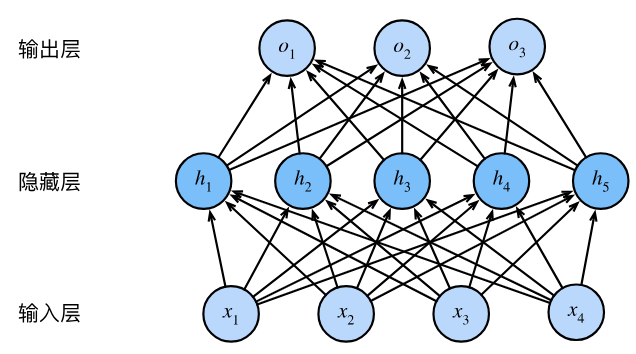
\includegraphics[width=0.6\textwidth]{4.1_1}
		\caption{隐藏层的加入}
		\label{fig:1}
	\end{figure}
	
	如同之前的章节一样,我们通过矩阵 $\bm{X} \in \mathbb{R}^{n \times d}$ 来表示 $n$ 个样本的小批量,其中每个样本具有 $d$ 个输入特征。对于具有 $h$ 个隐藏单元的单隐藏层多层感知机,用 $\bm{H} \in \mathbb{R}^{n \times h}$ 表示隐藏层的输出,称为隐藏表示(hidden representations)。在数学或代码中,$\bm{H}$ 也被称为隐藏层变量(hidden-layer variable)或隐藏变量(hidden variable)。因为隐藏层和输出层都是全连接的,所以我们有隐藏层权重 $\bm{W}^{(1)} \in \mathbb{R}^{d \times h}$ 和隐藏层偏置 $\bm{b}^{(1)} \in \mathbb{R}^{1 \times h}$ 以及输出层权重 $\bm{W}^{(2)} \in \mathbb{R}^{h \times q}$ 和输出层偏置 $\bm{b}^{(2)} \in \mathbb{R}^{1 \times q}$。形式上,我们按如下方式计算单隐藏层多层感知机的输出 $\bm{O} \in \mathbb{R}^{n \times q}$:
	$$
	\bm{H} = \bm{X} \bm{W}^{(1)} + \bm{b}^{(1)},
	$$
	$$
	\bm{O} = \bm{H} \bm{W}^{(2)} + \bm{b}^{(2)}.
	$$
	
	这其实还是仿射变换,并没有得到任何改进,我们可以证明这一等价性,即对于任意权重值,我们只需合并隐藏层,便可产生具有参数 $\bm{W} = \bm{W}^{(1)} \bm{W}^{(2)}$ 和 $\bm{b} = \bm{b}^{(1)} \bm{W}^{(2)} + \bm{b}^{(2)}$ 的等价单层模型:
	$$
	\bm{O} = (\bm{X} \bm{W}^{(1)} + \bm{b}^{(1)}) \bm{W}^{(2)} + \bm{b}^{(2)} = \bm{X} \bm{W}^{(1)} \bm{W}^{(2)} + \bm{b}^{(1)} \bm{W}^{(2)} + \bm{b}^{(2)} = \bm{X} \bm{W} + \bm{b}.
	$$
	
	为了发挥多层架构的潜力,我们还需要在仿射变换之后对每个隐藏单元应用非线性的激活函数(activation function)$\sigma$。激活函数的输出(例如,$\sigma(\cdot)$)被称为活性值(activations):
	$$
	\bm{H} = \sigma(\bm{X} \bm{W}^{(1)} + \bm{b}^{(1)}),
	$$
	$$
	\bm{O} = \bm{H} \bm{W}^{(2)} + \bm{b}^{(2)}.
	$$
	
	由于 $\bm{X}$ 中的每一行对应于小批量中的一个样本,出于记号习惯的考量,我们定义非线性函数 $\sigma$ 也以按行的方式作用于其输入,即一次计算一个样本。我们在 :numref:`subsec\_softmax\_vectorization` 中以相同的方式使用了 softmax 符号来表示按行操作。但是本节应用于隐藏层的激活函数通常不仅按行操作,也按元素操作。这意味着在计算每一层的线性部分之后,我们可以计算每个活性值,而不需要查看其他隐藏单元所取的值。对于大多数激活函数都是这样。
	
	为了构建更通用的多层感知机,我们可以继续堆叠这样的隐藏层,例如 $\bm{H}^{(1)} = \sigma_1(\bm{X} \bm{W}^{(1)} + \bm{b}^{(1)})$ 和 $\bm{H}^{(2)} = \sigma_2(\bm{H}^{(1)} \bm{W}^{(2)} + \bm{b}^{(2)})$,一层叠一层,从而产生更有表达能力的模型。
	
    根据万能逼近定理,我们甚至可以知道,这样的方式可以近似任何函数。\\
	
	\textbf{(2) 激活函数}
	
	\textbf{\textcircled{1} ReLU函数}
	
	最受欢迎的激活函数是修正线性单元(Rectified linear unit, ReLU),因为它实现简单,同时在各种预测任务中表现良好。ReLU 提供了一种非常简单的非线性变换,给定元素 $ x $,ReLU函数被定义为该元素与0的最大值:
	$$
	\text{ReLU}(x) = \max(x, 0).
	$$
	
	通俗地说,ReLU函数通过将相应的活性值设为0,仅保留正元素并丢弃所有负元素,并且是分段线性的。
	
	\begin{figure}[H]
		\centering
		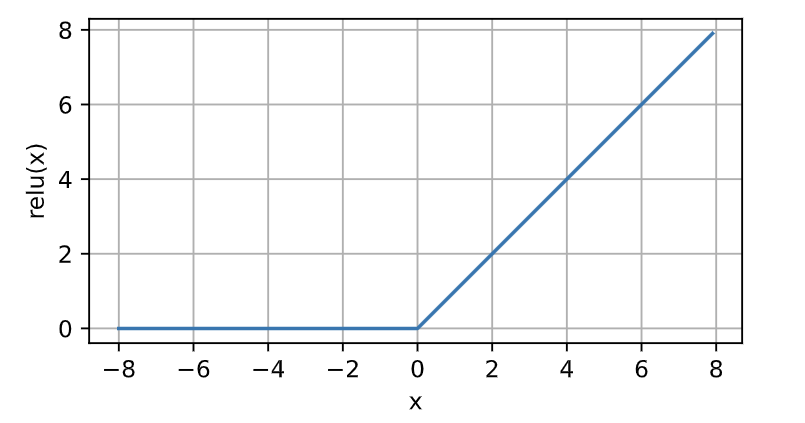
\includegraphics[width=0.6\textwidth]{4.1_2}
		\caption{ReLU函数}
		\label{fig:2}
	\end{figure}
	
	当输入为负时,ReLU 函数的导数为0,而当输入为正时,ReLU 函数的导数为1。 注意,当输入值精确等于 0 时,ReLU 函数不可导。 在此时,我们默认使用左侧的导数,即当输入为 0 时导数为 0。 我们可以忽略这种情况,因为输入可能永远都不会是 0.
	
	使用ReLU的原因是,它求导表现得特别好:要么让参数消失,要么让参数通过。这使得优化表现得更好,并且ReLU减轻了困扰以往神经网络的梯度消失问题。
	
	\textbf{\textcircled{2} sigmoid函数}
	
	[对于一个定义域在 $\mathbb{R}$ 中的输入,sigmoid函数将输入变换为区间(0, 1)上的输出]。因此,sigmoid通常称为挤压函数(squashing function):它将范围(-$\infty$, $\infty$) 中的任意输入压缩到区间 (0, 1) 中的某个值:
	$$
	\text{sigmoid}(x) = \frac{1}{1 + \exp(-x)}.
	$$
	
	该函数是一个平滑的、可微的阈值单元近似。当我们想要将输出视作二元分类问题的概率时,sigmoid仍然被广泛用作输出单元上的激活函数(sigmoid可以视为softmax的特例)。然而,sigmoid在隐藏层中已经较少使用,它在大部分时候被更简单、更容易训练的ReLU所取代。在后面关于循环神经网络的章节中,我们将描述利用sigmoid单元来控制时序信息流的架构。
	\begin{figure}[H]
		\centering
		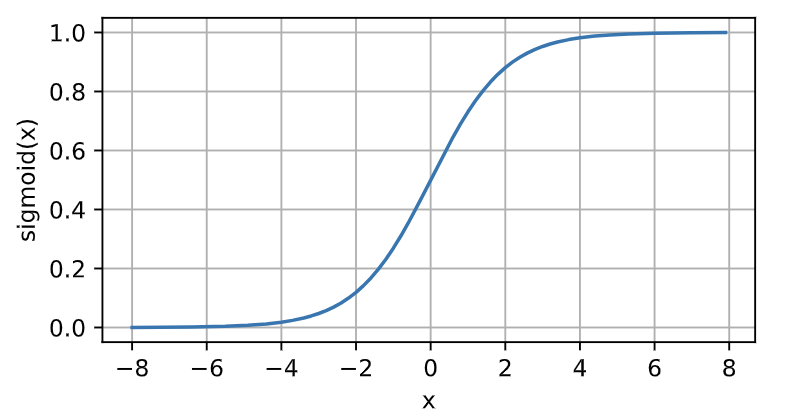
\includegraphics[width=0.6\textwidth]{4.1_3}
		\caption{sigmoid函数}
		\label{fig:3}
	\end{figure}
	
	sigmoid 函数的导数为下面的公式:
	$$
	\frac{d}{dx} \text{sigmoid}(x) = \frac{\exp(-x)}{(1 + \exp(-x))^2} = \text{sigmoid}(x) (1 - \text{sigmoid}(x)).
	$$
	
	\textbf{\textcircled{3} tanh函数}
	
	与sigmoid函数类似,[tanh(双曲正切)函数也能将其输入压缩转换到区间(-1, 1)上]。tanh函数的公式如下:
	$$
	\tanh(x) = \frac{1 - \exp(-2x)}{1 + \exp(-2x)}.
	$$
	
	下面我们绘制tanh函数。注意,当输入在0附近时,tanh函数接近线性变换。函数的形状类似于sigmoid函数,不同的是tanh函数关于坐标系原点中心对称。
	\begin{figure}[H]
		\centering
		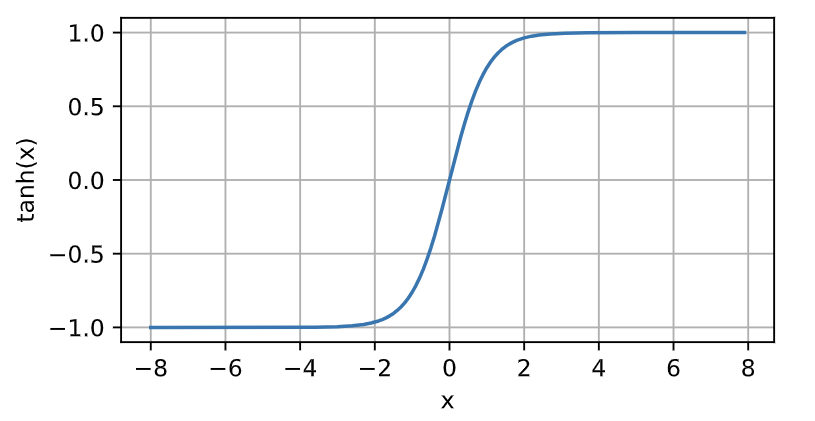
\includegraphics[width=0.6\textwidth]{4.1_4}
		\caption{tanh函数}
		\label{fig:4}
	\end{figure}
	
	\newpage
	\textbf{(3) 问题解答}
	
	\textbf{2、增加迭代周期的数量。为什么测试精度会在一段时间后降低?我们怎么解决这个问题?}
	
	\noindent \textbf{解}:
	
\end{document}